\documentclass{uebblatt}

\begin{document}

\maketitle{6}{}

\begin{aufgabe}{Morphismen zwischen fasernden Approximationen}
Seien~$X$ und~$X'$ Objekte einer Modellkategorie. Wähle fasernde
Approximationen~$r : X \to RX$ und~$r' : X' \to RX'$. Seien~$f$ und~$g$
Morphismen~$X \to X'$. Zeige: Wenn~$r' \circ f$ und~$r' \circ g$ zueinander
rechtshomotop sind, so sind auch die induzierten Morphismen~$Rf, Rg : RX \to
RX'$ zueinander rechtshomotop.
\end{aufgabe}

\begin{aufgabe}{Ein Kriterium für Identifizierung rechtshomotoper Morphismen}
Sei~$\M$ eine Modellkategorie und~$\C$ eine beliebige Kategorie. Sei~$F : \M_c
\to \C$ ein Funktor, der azyklische Kofaserungen auf Isomorphismen schickt.
Zeige, dass~$F$ rechtshomotope Morphismen identifiziert.
\end{aufgabe}

\begin{aufgabe}{Eigenschaften von Scheibenkategorien}
Sei~$M$ eine Modellkategorie. Sei~$A$ ein Objekt von~$M$. Zeige:
\begin{enumerate}
\item Ist~$M$ links- oder rechtseigentlich, so auch~$M/A$.
\item Ist~$M$ kofasernd erzeugt, so auch~$M/A$.
\end{enumerate}
\end{aufgabe}

\begin{aufgabe}{Lokale Präsentierbarkeit von Prägarbenkategorien}
Sei~$\C$ eine kleine Kategorie. Sei~$y : \C \hookrightarrow \PSh(\C)$ die
Yoneda-Einbettung in die Kategorie der Funktoren~$\C^\op \to \Set$.
Folgende Aussagen sind alle wahr. Zeige so viele
du möchtest.
\begin{enumerate}
\item Die Kategorie~$\PSh(\C)$ ist kovollständig.
\item Darstellbare Prägarben -- solche der Form~$y(X)$ für ein~$X \in \C$ --
sind~$\aleph_0$-kompakt.
\item Jede Prägarbe~$F$ ist ein kleiner Kolimes von darstellbaren Prägarben,
und zwar gilt etwas genauer~$F = \colim_{s \in F(X), X \in \C} y(X)$.
\item Die Kategorie~$\PSh(\C)$ ist lokal endlich-präsentierbar.
\end{enumerate}
\end{aufgabe}

\begin{aufgabe}{Regularität unendlich großer Nachfolgerkardinalzahlen}
Sei~$\kappa$ der Nachfolger einer unendlich großen Kardinalzahl.
Zeige, dass~$\kappa$ regulär ist.
\end{aufgabe}

\vfill
\centering
\href{http://spikedmath.com/182.html}{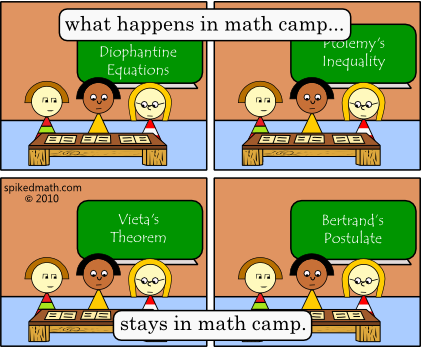
\includegraphics[height=4.9cm]{images/what-happens-in-math-camp}}
\quad
\href{http://smbc-comics.com/index.php?id=1777}{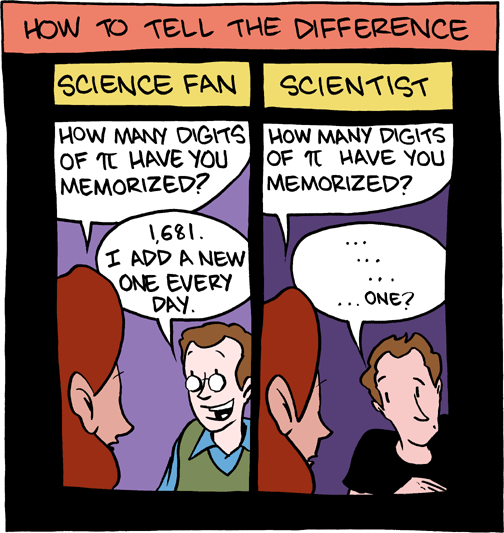
\includegraphics[height=4.9cm]{images/memorizing-pi}}
\par

\end{document}
